\chapter{Results}

This section presents the detailed findings and results of our experiments using various unsupervised anomaly detection models for the task of identifying faulty solder joints in \gls{pcb}. The models which we have evaluated here are PatchCore(section \ref{subsec:patchcore}), \gls{dfm}(section \ref{subsec:dfm}), \gls{dfkde}(section \ref{subsec:dfkde}), EfficientAD(section \ref{subsec:efficientad}), FastFlow(section \ref{subsec:fastflow}), which uses different hyperparameters, feature extraction backbones and its layers. We aim to study the effectiveness of these models in comparison to the current baseline models used by Siemens \gls{yolo}(section \ref{subsec:yolo}) while also the factors affecting their performances.

\section{Overall Performance of Models}

The table \ref{tab:overall model accuracy} and the bar chart \ref{fig:bar chart models accruacy} represent each model's overall accuracy performance, giving an initial overview of how these models compare in terms of how they classify anomalies correctly.

\begin{table}[ht!]
    \centering
    \begin{tabular}{|l|l|}
        \hline
        \textbf{Model} & \textbf{Accuracy} \\ \hline
        \textbf{Yolov8-L} & \textbf{95\%} \\ \hline
        \textbf{Yolov8-M} & \textbf{93.75\%} \\ \hline
        \textbf{PatchCore} & \textbf{91.25\%} \\ \hline
        Deep Feature Modeling(DFM) & 72.85\% \\ \hline
        Deep Feature Kernel Density Estimation(DFKDE) & 70.71\% \\ \hline
        FastFlow & 66.87\% \\ \hline
        EfficientAD & 60\% \\ \hline
    \end{tabular}
    \caption{Overall comparison of different models accuracy}
    \label{tab:overall model accuracy}
\end{table}

The chart \ref{fig:bar chart models accruacy} provides a graphical representation of the same data of each model's accuracy, where we can clearly visualize the performance of different models. As can be seen in table \ref{tab:overall model accuracy} and bar chart \ref{fig:bar chart models accruacy} the baseline model \gls{yolo}v8-L achieves the highest accuracy of 95\%, while the best performing unsupervised model is PatchCore closely following with an accuracy of 91.25\%, with only a 2.5\% difference in the accuracy of different size of baseline model \gls{yolo}v8-M. Other models, such as \gls{dfm}, \gls{dfkde}, FastFlow, and EfficientAD, show moderate performance. Here, none of the unsupervised anomaly detection models could overtake the supervised baseline model; one of the reasons for this is that the baseline model was trained in a supervised fashion, where it had access to all the labels of the image dataset. Whereas the anomaly detection models were not given any labels for the images, and while training, only anomaly free data was used, it had to figure out on its own which images were anomalous and which images were normal.

\begin{figure}[ht!]
    \centering
    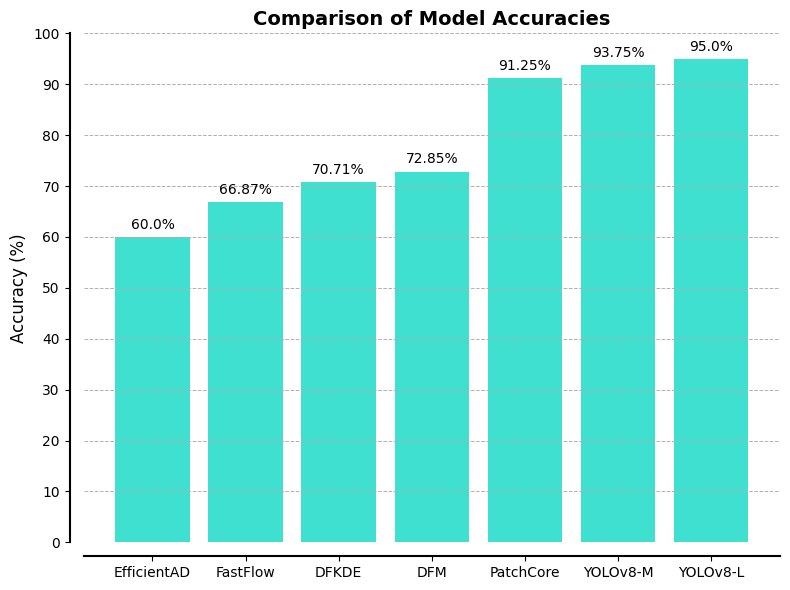
\includegraphics[width=1.1\linewidth]{Rohit_Master_Thesis//Images/bar_chart_model_acc.png}
    \caption{Bar chart representation of the different models accuracy like \gls{yolo}(baseline), our approach including PatchCore, \gls{dfm}, \gls{dfkde}, FastFlow, and EfficientAD.}
    \label{fig:bar chart models accruacy}
\end{figure}

\section{Model-wise breakdown of results}

\subsection*{PatchCore}

\begin{figure}[H]
    \centering
    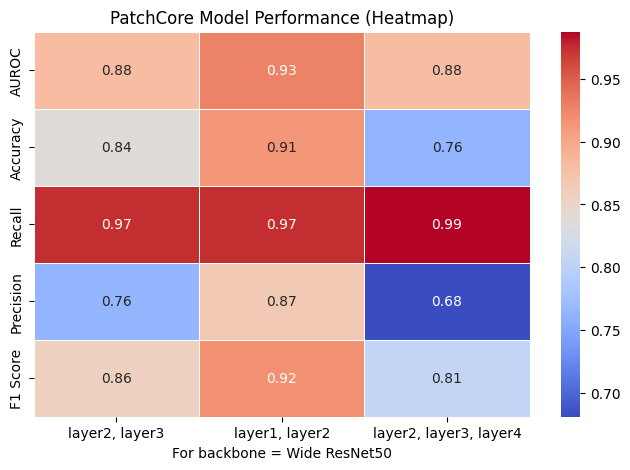
\includegraphics[width=1\linewidth]{Rohit_Master_Thesis//Images/patchcore heatmap.png}
    \caption{PatchCore heatmap for the experiment where backbone "Wide Resnet50" and layers "2, 3" were used.}
    \label{fig:patchcore heatmap}
\end{figure}

\iffalse
\begin{figure}[ht!]
    \centering  
    % First image
    \begin{minipage}{0.6\textwidth}
        \centering
        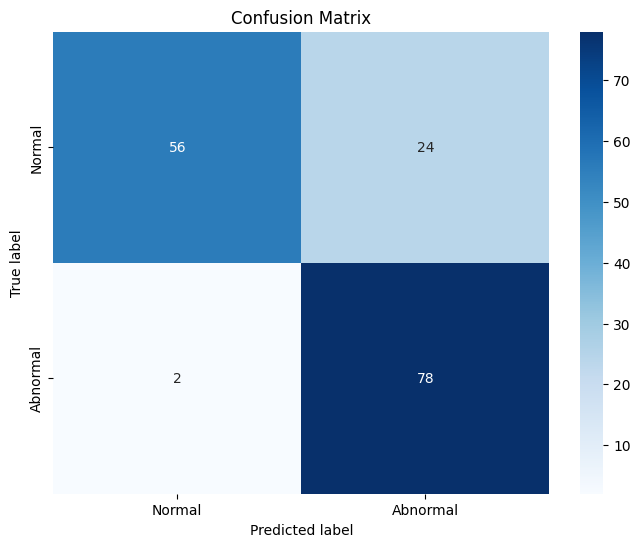
\includegraphics[width=\textwidth]{Rohit_Master_Thesis//Images/patchcore_config1_confusion_matrix.jpg} % Add your image file name here
        \caption{Configuration 1}
    \end{minipage}
    
    \vspace{0.5cm} % Adds vertical space between images
    
    % Second image
    \begin{minipage}{0.6\textwidth}
        \centering
        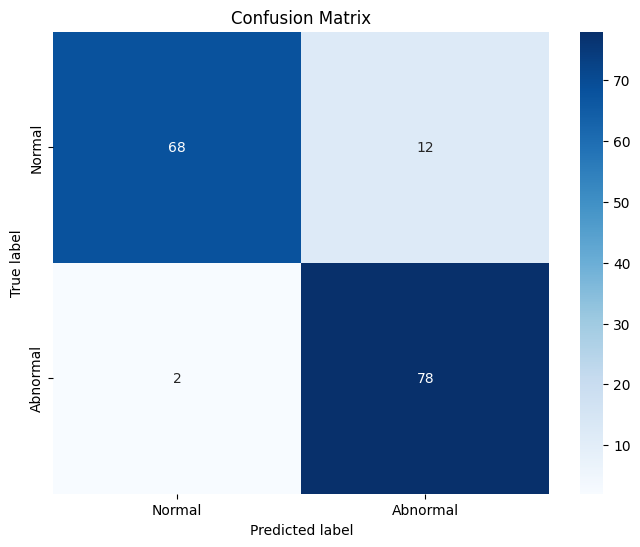
\includegraphics[width=\textwidth]{Rohit_Master_Thesis//Images/patchcore_config2_confusion_matrix.jpg} % Add your image file name here
        \caption{Configuration 2}
    \end{minipage}
    
    \vspace{0.5cm} % Adds vertical space between images
    
    % Third image
    \begin{minipage}{0.6\textwidth}
        \centering
        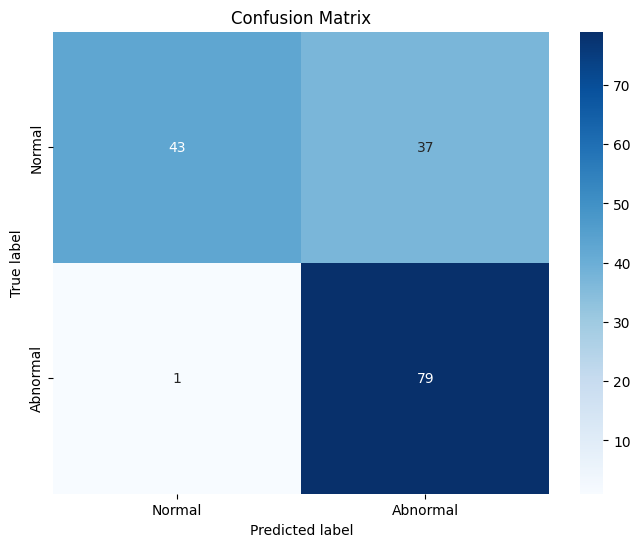
\includegraphics[width=\textwidth]{Rohit_Master_Thesis//Images/patchcore_config3_confusion_matrix.jpg} % Add your image file name here
        \caption{Configuration 3}
    \end{minipage}
    
    \caption{Comparison of Confusion Matrices for Different Configurations.}
    \label{fig:dataset-NG}
\end{figure}
\fi

For this experiment, we employed PatchCore with \texttt{wide\_resnet50\_2} backbone as feature extraction for performing anomaly detection. Firstly, the model extracts feature representations from specific layers of the backbone and then compares the patch-level features of test images with those stored in a memory bank built from normal data. PatchCore uses \gls{k-nn} retrieval for detecting deviations from nominal behavior by calculating the anomaly score based on the distance between patches from the test image and their closest counterparts in the memory bank. This allows PatchCore to perform well when the labeled data is not abundantly available. This model is explained in more detail in \ref{subsec:patchcore}.

For the first configuration, we have used backbone \texttt{wide\_resnet50\_2} with layer2 and layer3 as shown in the heatmap \ref{fig:patchcore heatmap}. This configuration achieves an \gls{auroc} score of 0.8816 and an overall accuracy of 83.75\%. The F1-score was relatively strong at 0.8571, suggesting that the model maintained a balance between precision and recall. The model had a precision of 0.7647, suggesting that sometimes the model classified normal data as anomalous, which resulted in moderate occurrence of false positives, as can be confirmed by the confusion matrix \ref{fig:patchcore config1 confusion matrix}. Whereas the high recall value of 0.975 indicates that the model was highly accurate in detecting almost all the anomalies as anomalies, with some false negatives, as can be seen in the \ref{fig:patchcore config1 confusion matrix}.

\begin{figure}[ht!]
    \centering
    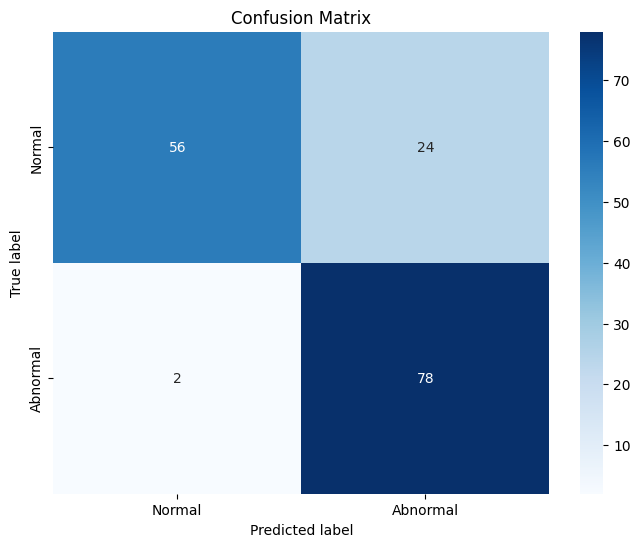
\includegraphics[width=1\linewidth]{Rohit_Master_Thesis//Images/patchcore_config1_confusion_matrix.jpg}
    \caption{Confusion matrix for the first configuration where backbone "Wide Resnet50" and layers "2, 3" were used.}
    \label{fig:patchcore config1 confusion matrix}
\end{figure}

The second configuration resulted in the best overall performance across all metrics, where the feature extraction was carried out by layer1 and layer2 of the same backbone \texttt{wide\_resnet50\_2}. This configuration resulted in a high \gls{auroc} score of 0.9271, with a significant increase in accuracy of 91.25\% as shown in the heatmap \ref{fig:patchcore heatmap}. We also saw improvement in F1-score by about 6.6\% from the previous configuration, reaching 0.9176, indicating an even better balance between precision and recall. The precision improved to 0.8667, indicating a reduction in false positives as seen in the confusion matrix \ref{fig:patchcore config2 confusion matrix} where the false positives were reduced by 50\% from the first configuration. While the recall remained high but the same as the first configuration at 0.975, meaning the model continued to detect almost all anomalies, as shown in the figure \ref{fig:patchcore config2 confusion matrix}. The improved performance of this configuration can be due to the use of features from the combination of layer 1 and layer 2, which incorporates the combination of both low-level and mid-level features. Low-level features might allow the model to detect fine-grained details, while layer 2 might provide the more complex structures needed to detect anomalies. These features can provide a richer, more detailed representation of normal data, making the detection of anomalies without overfitting normal data easier.

\begin{figure}[ht!]
    \centering
    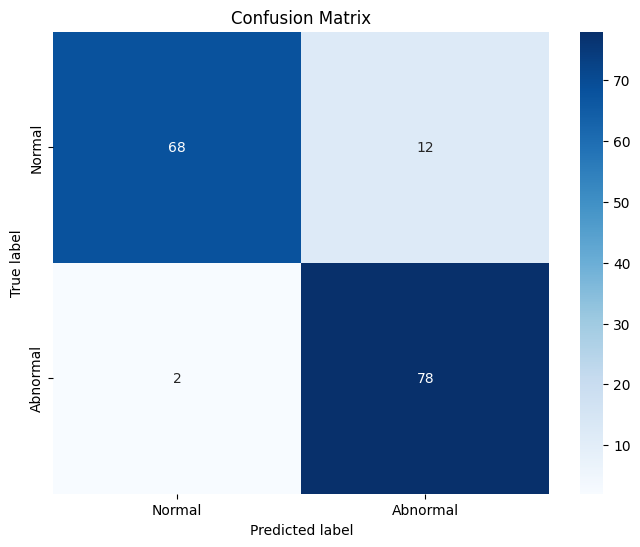
\includegraphics[width=1\linewidth]{Rohit_Master_Thesis//Images/patchcore_config2_confusion_matrix.jpg}
    \caption{Confusion matrix for the second configuration where backbone "Wide Resnet50" and layers "1, 2" were used.}
    \label{fig:patchcore config2 confusion matrix}
\end{figure}

In the third configuration, layer 2, layer 3, and layer 4 were used for the backbone \texttt{wide\_resnet50\_2}, it resulted in a lower \gls{auroc}score of 0.8807 which is almost equal to the \gls{auroc} score for first configuration, and the accuracy we got is 76.25\% which is the lowest of all the configuration. The F1-score also decreased slightly to 0.8061 due to a drop in precision value to 0.6810. This lower precision indicates that the model produced a higher number of false positives, i.e., more normal images were classified as anomalous, as can be seen in confusion matrix \ref{fig:patchcore config3 confusion matrix} where out of 80 normal images, 37 were classified as anomalous. However, the recall was the highest at 0.9875, which means that the model was still able to detect almost all of the anomalies, as seen in the figure \ref{fig:patchcore config3 confusion matrix} out of 80, 79 were correctly classified as anomalous with only one being misclassified as normal. The inclusion of deeper layers, like layer 4, probably introduced more abstract features, which may have been less effective for the detection of fine-grained anomalies, resulting in the reduction of overall performance. This configuration highlights the importance of extraction of features from appropriate layers for ensuring balance between detecting true anomalies and avoiding excessive false positives.

\begin{figure}[ht!]
    \centering
    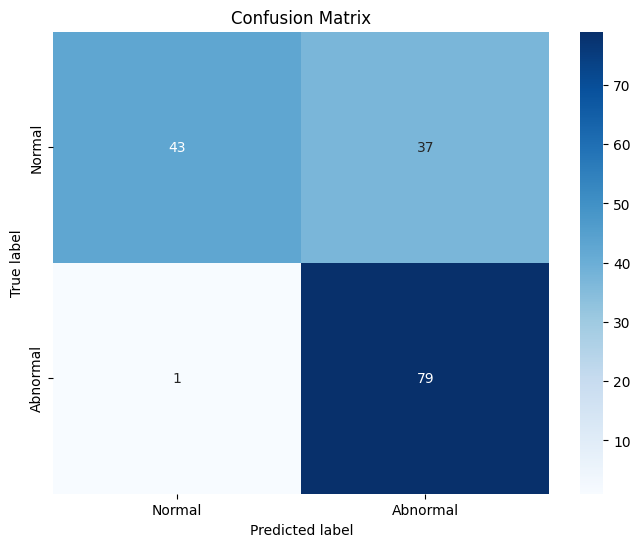
\includegraphics[width=1\linewidth]{Rohit_Master_Thesis//Images/patchcore_config3_confusion_matrix.jpg}
    \caption{Confusion matrix for the third configuration where backbone "Wide Resnet50" and layers "2, 3, 4" were used.}
    \label{fig:patchcore config3 confusion matrix}
\end{figure}

\subsection*{\gls{yolo}}

Two different model sizes of \gls{yolo}v8 \cite{Ultralytics2024} were evaluated for this experiment: \gls{yolo}v8-M(medium) and \gls{yolo}v8-L(large). Both the models were trained for 200 epochs on the training dataset.

The \textbf{\gls{yolo}v8-L} model, which is larger and more complex, reached an accuracy of 95\% after 200 epochs. The model's high accuracy could be due to its increase in the depth and number of parameters, which allows it to capture more detailed and complex patterns in the dataset. Also it being a supervised model, having access to all the labels while training helps it to learn better and fit the model well to the data.

\begin{figure}
    \centering
    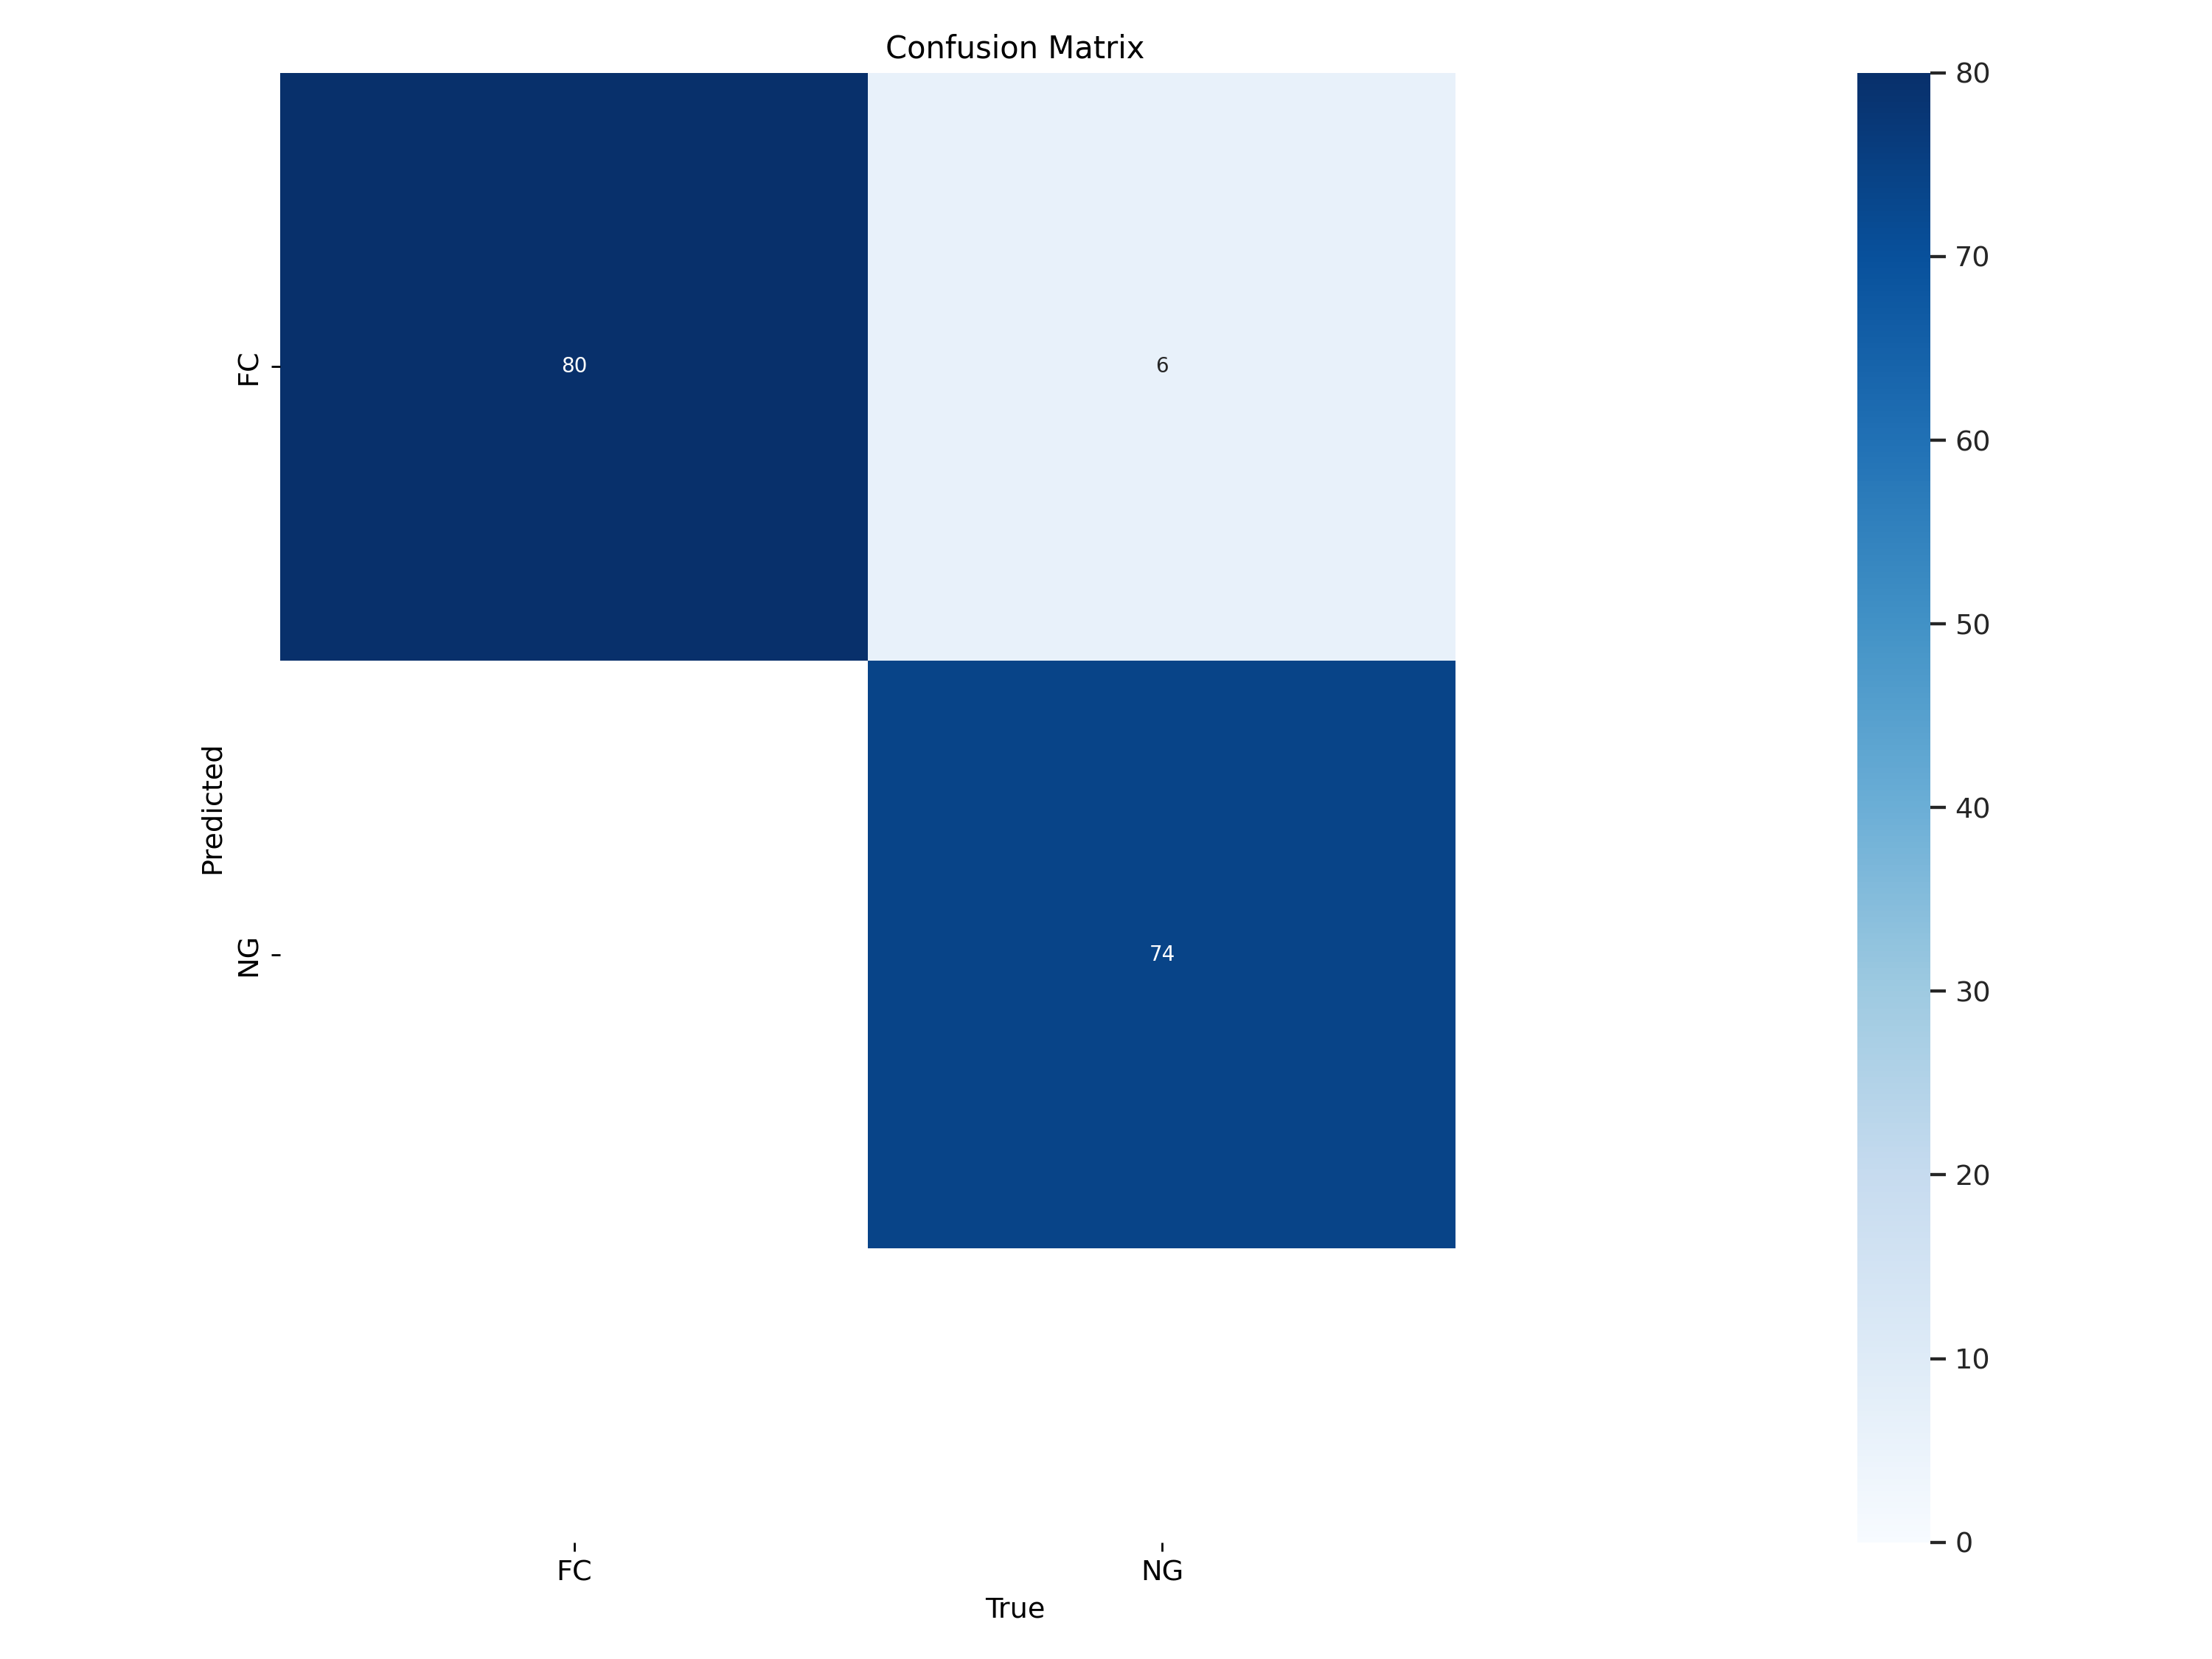
\includegraphics[width=1.3\linewidth]{Rohit_Master_Thesis//Images/yolov8l_confusion_matrix.png}
    \caption{Confusion matrix for the baseline model \gls{yolo}v8-L, its accuracy is 95\%}
    \label{fig:yolov8l confusion matrix}
\end{figure}

The confusion matrix, as shown in figure \ref{fig:yolov8l confusion matrix}, provides a more detailed look into how well the model performs in the classification task. We can see that the model was able to correctly classify all the normal(FC) images as normal. While only 6 were false positives, i.e., anomalous(NG) images were classified as normal images, the rest of the 74 were correctly classified as NG, i.e., True Negatives. These values are consistent with the precision, recall, and F1-score results as shown in table \ref{tab:yolov8_performance}. The precision of 1.0 highlights the model's reliability in predicting normal(FC) instances, as it did not make any incorrect predictions for that class. The recall of 0.925, while still quite good, indicates that the model misclassified a small number of anomalous(NG) as normal(FC). With the impressive F1-score of 0.9615, shows the models well-rounded performance.

\begin{table}[ht!]
    \centering
    \begin{tabular}{|c|c|c|c|c|}
        \hline
        \textbf{Model} & \textbf{Accuracy} & \textbf{Precision} & \textbf{Recall} & \textbf{F1-score} \\ \hline
        \textbf{YOLOv8-M} & 93.75\% & 0.9867 & 0.925 & 0.9547 \\ \hline
        \textbf{YOLOv8-L} & 95\% & 1.0 & 0.925 & 0.9615 \\ \hline
    \end{tabular}
    \caption{Comparison of YOLOv8-M and YOLOv8-L Model Performance}
    \label{tab:yolov8_performance}
\end{table}

%Probably for discussion section(remember to paraphrase)
%Explanation of Results
%The performance of YOLOv8-L is in line with its design as a larger, more powerful model. The depth and complexity of the YOLOv8-L architecture allow it to capture a wide variety of patterns and features in the data, leading to its high precision and recall. The non-maximum suppression (NMS) technique used in YOLOv8 helps further refine the predictions by ensuring that overlapping bounding boxes are filtered, resulting in more accurate object classification. Additionally, YOLOv8-L's anchor-free detection mechanism improves its ability to generalize across objects of various sizes, contributing to its robustness in detecting NG and FC items.

The \textbf{\gls{yolo}v8-M} model, which is smaller and more lightweight when compared to \gls{yolo}v8-L, reaches an accuracy of 93.75\%. This is slightly lower than its bigger model, as seen from the table \ref{tab:yolov8_performance}, but its overall performance was still quite impressive.

\begin{figure}[ht!]
    \centering
    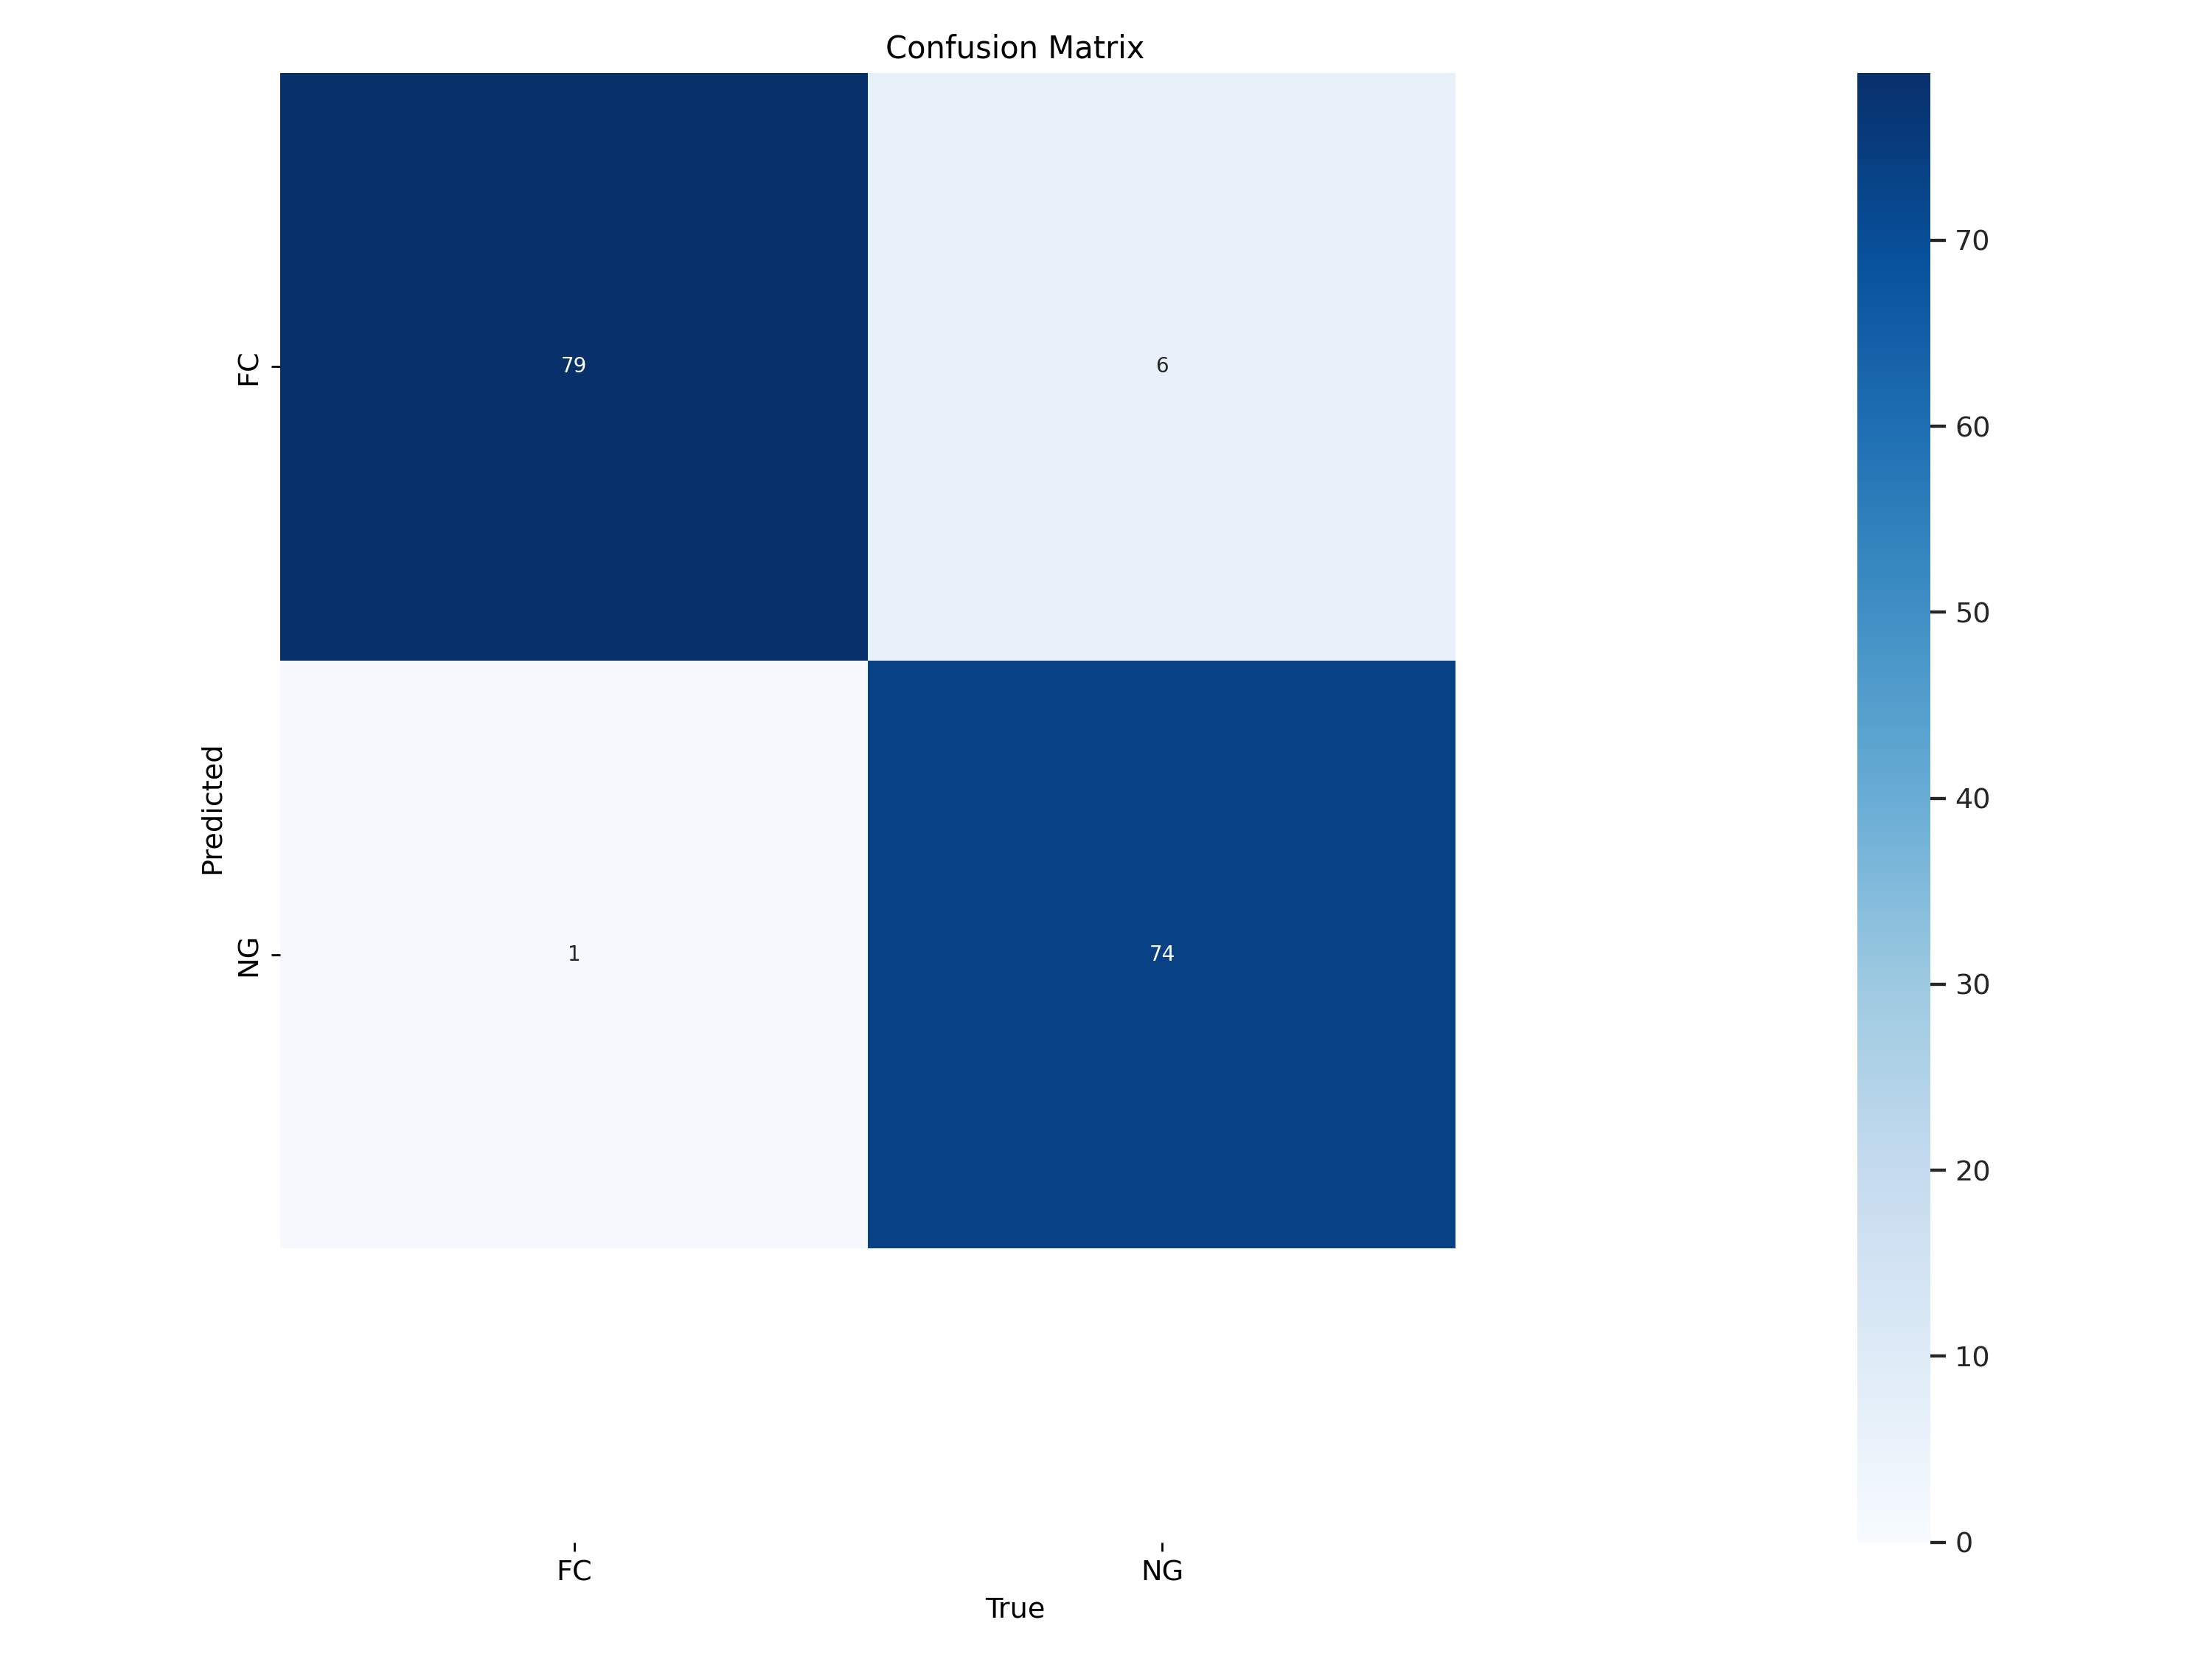
\includegraphics[width=1.3\linewidth]{Rohit_Master_Thesis//Images/yolov8m_confusion_matrix.png}
    \caption{Confusion matrix for the baseline model \gls{yolo}v8-M, its accuracy is 93.75\%}
    \label{fig:yolov8m confusion matrix}
\end{figure}

The confusion matrix in figure \ref{fig:yolov8m confusion matrix} shows almost similar results to that of \gls{yolo}v8-L. With 79 True positives and 74 true negatives, while only making 6 false positives and 1 false negative prediction, apart from the 1 misclassified normal image as anomalous, the results are similar to that of \gls{yolo}v8-L. This indicates that the performance of the \gls{yolo}v8-M, though highly accurate, still falls just short of \gls{yolo}v8-L's performance due to its smaller capacity for learning complex patterns. As can be seen from the table \ref{tab:yolov8_performance}, the model achieved a precision of 0.9867, meaning that almost all of the predictions of normal(FC) images were correct. The recall for both the \gls{yolo}v8-L and \gls{yolo}v8-M matches and is equal to 0.925, indicating that both models successfully detected the same number of FC cases. The F1-score of the model was 0.9547, which is slightly lower than \gls{yolo}v8-L due to the slight decrease in the precision. While the model was highly accurate, it did produce a small number of false positives, in this case, 6 anomalous(NG) images were misclassified as normal(FC), which reduced its precision slightly.

%See if you need to include loss and accuracy curve for both the models of YOLO

%Probably for discussion section(remember to paraphrase)
%Explanation of Results

%YOLOv8-M strikes a balance between computational efficiency and accuracy. The model achieves 93.75\% accuracy, which is competitive given its smaller architecture compared to YOLOv8-L. The slightly lower performance is expected due to YOLOv8-M’s reduced depth and number of parameters, which limits its ability to capture as many intricate patterns in the data as YOLOv8-L. However, YOLOv8-M’s simpler structure makes it faster and more computationally efficient, making it suitable for tasks where real-time performance and resource limitations are important.

%Model Comparison and Insights
%YOLOv8-L outperforms YOLOv8-M by achieving 95\% accuracy, compared to YOLOv8-M’s 93.75\%. This difference in performance can be attributed to the larger number of layers and parameters in YOLOv8-L, which allows it to capture more detailed features from the dataset. YOLOv8-L’s larger architecture is particularly beneficial for classification tasks that involve complex patterns or subtle differences between classes, making it a better choice for applications where accuracy is critical.

%However, YOLOv8-M offers significant advantages in terms of speed and computational efficiency. Despite having fewer layers, YOLOv8-M achieves strong results, making it a good option for scenarios where real-time inference is necessary or where computational resources are limited. The slight trade-off in accuracy is reasonable given the gains in efficiency, making YOLOv8-M ideal for environments where fast processing is prioritized over achieving the highest possible accuracy.

\subsection*{\gls{dfm}}

In this section, we will look into the results obtained from various experiments using \gls{dfm}. \gls{dfm} is explained in the section \ref{subsec:dfm}, and in our experiments, we evaluated \gls{dfm} performance using various backbones, their layers, and pooling techniques to explore the robustness and accuracy of the model. Below the results are divided based on the backbone used. 

\subsubsection*{ResNet50}

Here, we used ResNet50's layer4 for feature extraction along with \gls{nll} as the scoring type. This gave us the \gls{auroc} score of 0.6309 and F1-score of 0.6689, with an overall accuracy of 50.7\%, which is not very good, as can be seen from the table \ref{tab:dfm resnet results}, it is basically doing random guessing. The low F1-score suggests that while the model was good at detecting anomalies, it struggled with precision because of the high number of false positives. These findings suggest that using features extracted from higher layers, like layer 4, may have led the model to focus on more abstract, high-level features that are less effective at determining anomalies from normal samples.

\begin{table}[ht!]
    \centering
    \begin{tabular}{|l|c|c|c|c|c|}
        \hline
        \textbf{Model} & \textbf{Accuracy (\%)} & \textbf{\gls{auroc}} &\textbf{Precision} & \textbf{Recall} & \textbf{F1-score} \\ \hline
        ResNet50 & 50.71\% & 0.6309 & 0.5036 & 1.0 & 0.6699 \\ \hline
        Wide-ResNet50-2 (layer2, nll) & 60\% & 0.6382 & 0.5556 & 1.0 & 0.7143 \\ \hline
        Wide-ResNet50-2 (layer2, fre) & 62.12\% & 0.5795 & 0.5681 & 1.0 & 0.7254 \\ \hline
        Wide-ResNet50-2 (layer3) & 62.86\% & 0.7265 & 0.5738 & 1.0 & 0.7292 \\ \hline
    \end{tabular}
    \caption{Results for ResNet and Wide-ResNet50-2 Backbones}
    \label{tab:dfm resnet results}
\end{table}

Another configuration that we tried was using a different variant of ResNet50 called Wide-ResNet50-2 and performing feature extraction using layer 2 while keeping the \gls{pca} level at 0.97 and using \gls{nll} score type. This resulted in a slight improvement in both the accuracy and \gls{auroc} score of 60\% and 0.6382, respectively. The precision improved to 0.5556, while the recall stayed at 1.0, resulting in an F1-score of 0.7143, as shown in the table \ref{tab:dfm resnet results}. Along with that, we also performed a similar experiment by keeping the backbone and layer the same but changing the \gls{pca} level to 0.995 and scoring type to \gls{fre}. This resulted in much better compared to when we used scoring type as \gls{nll}, where accuracy increased by about 2\% to 62.12\% while seeing a drop in \gls{auroc} to 0.5795. The recall stayed the same at 1.0, but a slight increase in precision was observed to 0.5681, therefore increasing the F1-score to 0.7254. This improvement in both precision and F1-score shows that lower-level features from layer 2 were more effective at capturing variations between normal and anomalous images. Finally, after seeing better results with \gls{fre} scoring type, we experimented with one more layer of the same backbone. The layer used here was layer 3, and with this, we again saw slight improvement across all the metrics. The accuracy came out to be 62.86\% which is a small incremental update, while with \gls{auroc} score we saw an improvement of about 25\% when compared to Wide-ResNet50-2 (layer2, \gls{fre}) of the table \ref{tab:dfm resnet results}, and saw a rise of about 14\% when compared with Wide-ResNet50-2 (layer2, \gls{nll}). Other layers were also tried for both the ResNet50 and Wide-ResNet50-2 backbone, but all of them resulted in the model just randomly guessing the predictions, i.e., the accuracy was 50\%.

\subsubsection*{Densenet}

Next, we conducted experiments using different DenseNet backbones. Firstly, we used DenseNet121, which extracted features from the features.norm5 layer and the \gls{fre} score type. This configuration improved the model's performance further, with an \gls{auroc} score of 0.7309 and an accuracy of 61.43\%. The model reached a precision of 0.5645 and a recall of 1.0, giving an F1-score of 0.7216. These improved scores suggest that the DenseNet architecture, which relies on dense connections and feature reuse, contributed to improved feature representations for anomaly detection. Table \ref{tab:dfm densenet results} shows the results of different backbones of DenseNet.

\begin{table}[ht!]
    \centering
    \begin{tabular}{|l|c|c|c|c|c|}
        \hline
        \textbf{Model} & \textbf{AUROC} & \textbf{Accuracy} & \textbf{Precision} & \textbf{Recall} & \textbf{F1-score} \\ \hline
        DenseNet121 & 0.7310 & 0.6143 & 0.5645 & 1.0 & 0.7216 \\ \hline
        DenseNet169 (norm5) & 0.7456 & 0.6571 & 0.5932 & 1.0 & 0.7447 \\ \hline
        \textbf{DenseNet169 (denseblock3, 0.97 PCA)} & \textbf{0.7203} & \textbf{0.7286} & 0.6538 & 0.9714 & 0.7816 \\ \hline
        DenseNet169 (denseblock3, 0.995 PCA) & 0.7190 & 0.7214 & 0.6422 & 1.0 & 0.7821 \\ \hline
        DenseNet201 (denseblock3, 0.995 PCA) & 0.7259 & 0.7143 & 0.6389 & 0.9857 & 0.7753 \\ \hline
        %DenseNet264d (untrained) & 0.8029 & N/A & N/A & N/A & 0.8471 \\ \hline
        %DenseNet201 (denseblock3, 0.97 PCA) & 0.7265 & N/A & N/A & N/A & 0.8460 \\ \hline
    \end{tabular}
    \caption{Results for DenseNet Backbones}
    \label{tab:dfm densenet results}
\end{table}

The best performing configuration for the DenseNet architecture comes from the DenseNet169 backbone, with features extracted from features.denseblock3 layer, a \gls{pca} level of 0.97, and the \gls{fre} score type as shown in the table \ref{tab:dfm densenet results}. This configuration gave an \gls{auroc} score of 0.7203 and an accuracy of 72.86\%. Precision also improved to 0.6538. While recall reduced slightly, it remained high at 0.9714, resulting in an F1-score of 0.7816. This improvement in both the precision and the F1-score suggests that the DenseNet169's larger size allowed for better feature extraction and classification, particularly when extracting features from the third dense block. The high recall score indicates that the model was able to detect most of the anomalies, as can be seen in the confusion matrix \ref{fig:dfm densenet169 confusion matrix}, while the increase in precision value indicates a significant reduction in the number of false positives relative to other configurations.

\begin{figure}[ht!]
    \centering
    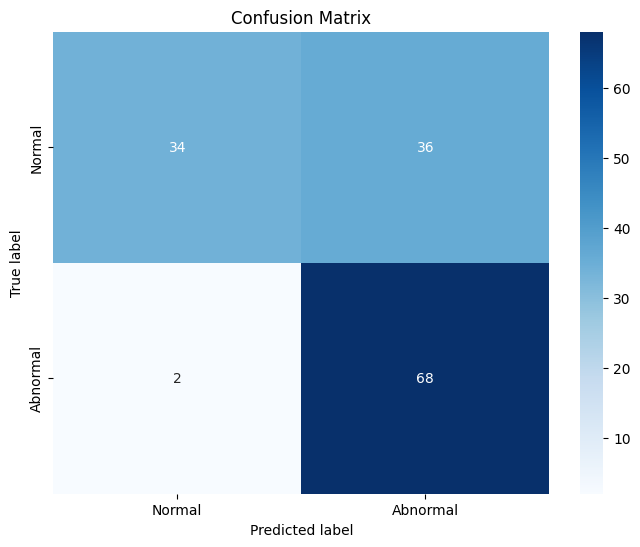
\includegraphics[width=1\linewidth]{Rohit_Master_Thesis//Images/dfm_densenet_best_confusion_matrix.png}
    \caption{Confusion matrix for the best performing configuration for \gls{dfm} model with DenseNet169 backbone, its accuracy is 72.86\%}
    \label{fig:dfm densenet169 confusion matrix}
\end{figure}

After getting good results with the configuration explained above, we thought of checking another variation of the DenseNet169 backbone while keeping the feature extraction layer and scoring type the same as before but using a higher \gls{pca} level of 0.995, allowing for a greater variance in the data. However, the results were more or less similar to the previous configuration, with a slightly lower \gls{auroc} of 0.7190 and an accuracy of 72.14\%, along with a precision of 0.6422 and an F1-score of 0.7821. The recall remained at 1.0, but the decrease in precision compared to the previous configuration indicates that the increased retained variance caused the model to classify a higher number of normal images as anomalous. Finally, DenseNet201 was also tested with the same feature extraction layer, keeping the other hyperparameters the same. This configuration also gave similar results to previous ones highlighted in the table \ref{tab:dfm densenet results}.


% In discussions explain also the difference between scoring type fre and nll
% In discussion also discuss why was the recall for most part 1.0

\subsection*{\gls{dfkde}}

Here, we discuss the results obtained for the model \gls{dfkde}. It combines the power of \gls{dl} with statistical methods like \gls{pca} and \gls{kde}. The model first extracts robust features using a pre-trained deep neural network, then reduces their dimensionality by using \gls{pca}, and finally applying \gls{kde} to model the distribution of normal data. Two backbones were tested in this experiment, namely ResNet18 and Wide-ResNet50. The overview of the results for different configurations in the form of a bar chart is shown in figure \ref{fig:dfkde model results}.

\begin{figure}[ht!]
    \centering
    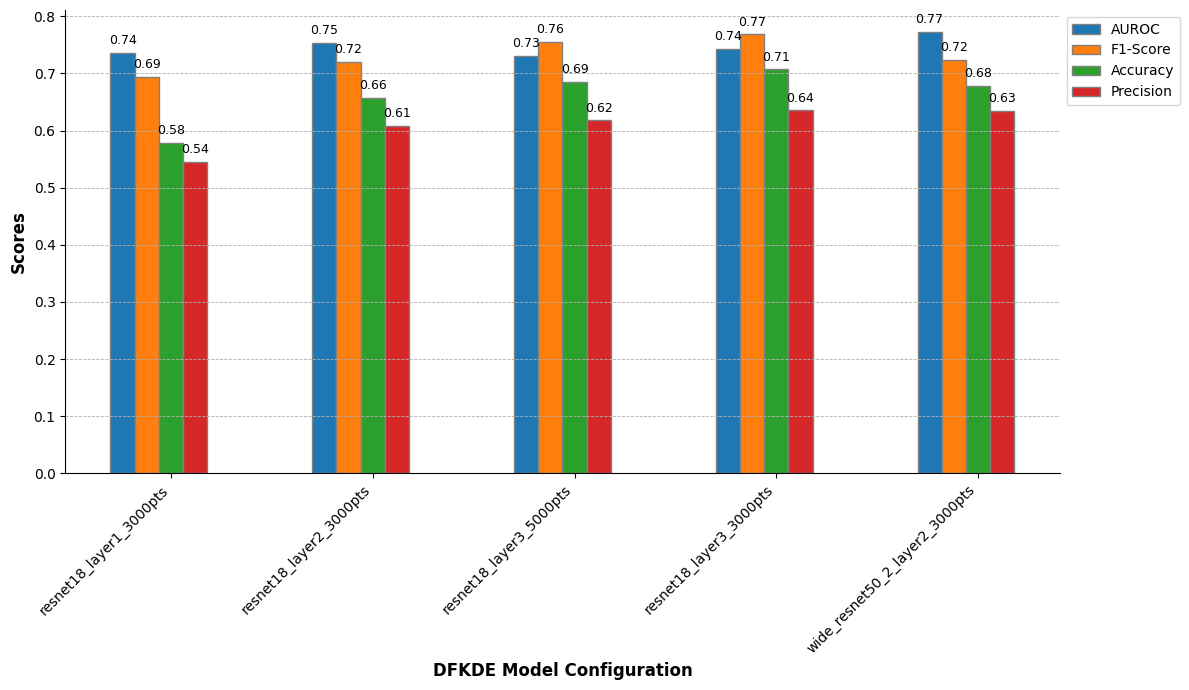
\includegraphics[width=1.2\linewidth]{Rohit_Master_Thesis//Images/dfkde_model_results.png}
    \caption{DFKDE model results for different backbones. The values shown here include \gls{auroc} score, F1-score, accuracy, and precision.}
    \label{fig:dfkde model results}
\end{figure}

\subsubsection*{ResNet18}

For the first experiment with the ResNet18 backbone, we use the feature extraction layer 1. This configuration aims at capturing the lower-level basic features and is trained with a maximum of 3000 training points to fit the \gls{kde} model.

Its results are shown in the table \ref{tab:dfkde resnet18 results}. As can be seen, the performance is not quite good, with \gls{auroc} score of 0.7364 and an accuracy of 57.86\%. Precision is quite low at 0.5447, while recall is high at 0.9571, resulting in an F1-score of 0.6943. The lower precision value indicates that the features extracted from the lower layer lead to the introduction of noise, leading to higher false positives. While the high recall value suggests that the model was still able to detect most of the anomalies correctly. However, the overall performance of the model still suffered as low-level features are less effective in anomaly detection for \gls{dfkde} model.

\begin{table}[ht!]
    \centering
    \begin{tabular}{|l|c|c|c|c|c|c|}
        \hline
        \textbf{Configuration} & \textbf{AUROC} & \textbf{Accuracy(\%)} & \textbf{Precision} & \textbf{Recall} & \textbf{F1-Score} \\ \hline
        Layer1, max training points 3000 & 0.7364 & 57.86\% & 0.5447 & 0.9571 & 0.6943 \\ \hline
        Layer2, max training points 3000 & 0.7535 & 65.71\% & 0.6078 & 0.8857 & 0.7209 \\ \hline
        Layer3, max training points 3000 & 0.7428 & 70.71\% & 0.6355 & 0.9714 & 0.7684 \\ \hline
        Layer3, max training points 5000 & 0.7310 & 68.57\% & 0.6182 & 0.9714 & 0.7556 \\ \hline
    \end{tabular}
    \caption{Results for DFKDE Model with ResNet18 Backbone}
    \label{tab:dfkde resnet18 results}
\end{table}

For the second experiment with the ResNet18 backbone, we used feature extraction layer 2, and the number of maximum data points for \gls{kde} model remained the same as before at 3000.

The model achieved an \gls{auroc} score of 0.7535, which is slightly better than when features were extracted from layer 1, an accuracy of 65,71\% is observed, which is about 14\% higher than that of configuration 1, as can be seen in the table \ref{tab:dfkde resnet18 results}. A precision of 0.6078 and a recall of 0.8857, resulting in an F1-score of 0.7209. This improvement in \gls{auroc} score and precision indicates that the mid-level features are more effective in anomaly detection for \gls{dfkde} model as they maintain the balance of the low-level details and high-level semantic information. Even though recall is slightly reduced compared to layer 1, the improvement in precision indicates a reduction in false positives.

For the third experiment, we select layer 3 for feature extraction of the backbone ResNet18, which is responsible for capturing higher-level semantic information. This layer offers a more abstract representation of the input data, which can be particularly suitable for anomaly detection tasks. This configuration was the best performing one in the \gls{dfkde} model.

As shown in the table \ref{tab:dfkde resnet18 results} an \gls{auroc} score of 0.7427, an accuracy of 70.71\% which is more than 22\% higher than configuration 1, and more than 7\% higher than configuration 2. A further improvement in precision was observed at 0.6355, and a recall of 0.9714, leading to an F1-score of 0.7684. The layer 3 features give more abstract representations of the data, which helped reduce false positive rates further while also maintaining high recall. However, a slight dip in \gls{auroc} compared to layer2 configuration can indicate that while the high-level features are useful, they might lack some of the finer details necessary for achieving good anomaly detection performance.

Next, for the fourth experiment, to examine the effects of increasing the number of training points, we increased the max training points parameter to 5000 points to fit the \gls{kde} model while keeping the backbone and the feature extraction layer the same as ResNet18 layer3. The goal was to see if more training data would improve \gls{kde}'s ability to model normal distribution, as layer 3 gave the best results.

In table \ref{tab:dfkde resnet18 results}, we can see that the model reached an \gls{auroc} score of 0.7310, with an accuracy of 68.57\%, which is lower than the third experiment, and with precision and recall of 0.6182 and 0.9714 respectively, leading to an F1-score of 0.7556. The performance was slightly worse than that of configuration 3, where layer 3 with 3000 max training points was used. This indicates that the number of training points may be less important than the layer from which the features are extracted, at least beyond a threshold.

\subsubsection*{Wide-ResNet50}

The second backbone we experimented with was Wide-ResNet50-2, which is a wider version of the standard ResNet50 architecture. In this experiment, features were extracted using layer 2 of the backbone. This configuration was chosen because the middle layer performed better for the ResNet18 backbone experiments and with the wider architecture, which can capture more detailed feature representations, which could possibly improve the anomaly detection performance.

\begin{table}[ht!]
    \centering
    \begin{tabular}{|l|c|c|c|c|c|c|}
        \hline
        \textbf{Configuration} & \textbf{AUROC} & \textbf{Accuracy(\%)} & \textbf{Precision} & \textbf{Recall} & \textbf{F1-Score} \\ \hline
        Layer2, max training points 3000 & 0.7725 & 67.86\% & 0.6344 & 0.8429 & 0.7239 \\ \hline
    \end{tabular}
    \caption{Results for DFKDE Model with Wide-ResNet50-2 Backbone}
    \label{tab:dfkde wide-resnet50 results}
\end{table}


This configuration showed improved performance in \gls{auroc} score and precision as seen from the table \ref{tab:dfkde wide-resnet50 results} of 0.7725 and 0.6344, respectively. The accuracy was 67.86\%, and the recall fell to 0.8429, resulting in the F1-score of 0.7239. The wider architecture and mid-level features from layer 2 did help the model capture more subtle patterns in the data, which resulted in a higher \gls{auroc} score when compared to ResNet18 experiments. The precision also slightly improved, indicating that the model was comparatively more accurate in detecting true anomalies. However, the lowest recall value of all the experiments combined from resNet18 and Wide-ResNet50 indicates that the model became slightly less sensitive to anomalies, likely as a result of the increase in specificity brought by the wider backbone.

\subsection*{FastFlow}

For this experiment, we used the FastFlow model with ResNet18, Wide-ResNet50-2, \gls{deit}, \gls{cait} as backbones for feature extraction. An overview of all the results is shown in the form of a bar chart in the figure \ref{fig:fastflow model results}. The best performing configuration in terms of accuracy was the one where \gls{deit} architecture was used for feature extraction, achieving 66.87\%. Below, we will discuss all the experiments and their results in detail, grouped based on the backbones used. Here, all the models were trained for 50 epochs except for when callback functionality was used. Then, it is trained until a condition is met.

\begin{figure}[H]
    \centering
    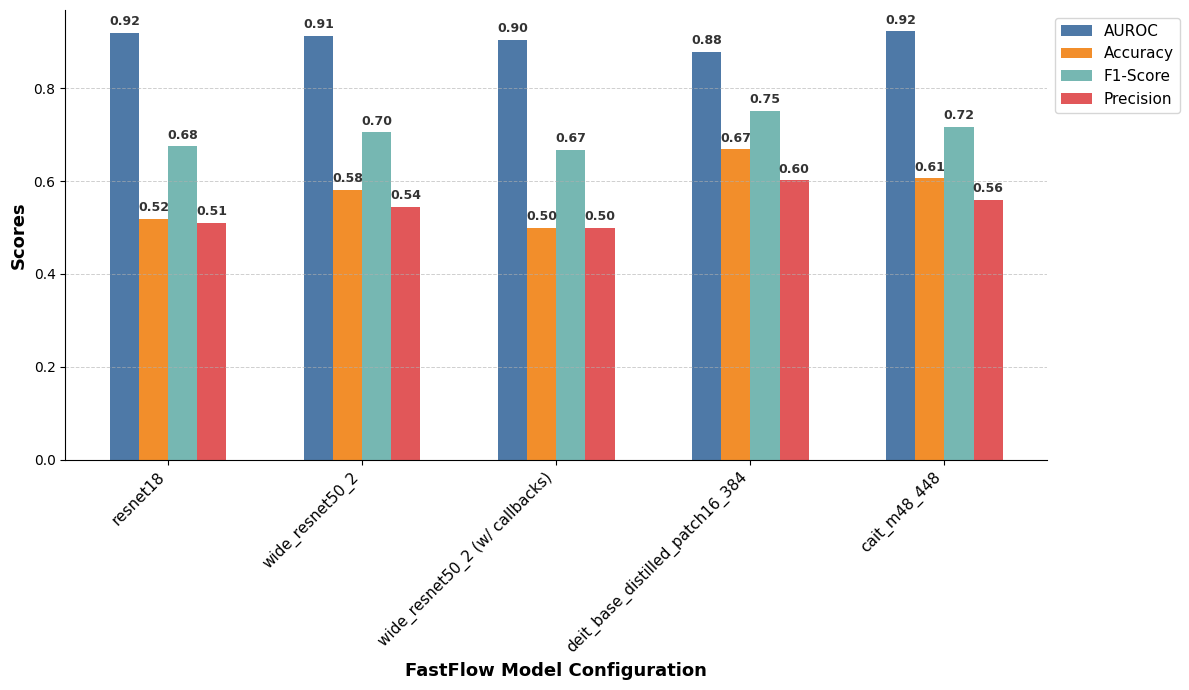
\includegraphics[width=1.2\linewidth]{Rohit_Master_Thesis//Images/fastflow_model_results.png}
    \caption{FastFlow model's results bar-chart for different configurations and backbones used for feature extraction.}
    \label{fig:fastflow model results}
\end{figure}

\subsubsection*{ResNet18}

For the first experiment, we have used ResNet18 as the backbone for feature extraction. This configuration achieved an \gls{auroc} score of 0.9199, which is quite good, and it demonstrates the models effectiveness in distinguishing normal images from abnormal ones on training and testing dataset. But, the overall accuracy on the unseen custom dataset is as good as random guessing, equating to 51.88\%, reflecting imbalanced classification performance, as shown in the table \ref{tab:fastflow resnet18}. The recall of 1.0 shows that the model was able to detect all anomalous instances. However, the precision was low, at 0.5096, giving an F1 score of 0.6751. 

\begin{table}[ht!]
    \centering
    \begin{tabular}{|l|c|c|c|c|c|}
        \hline
        \textbf{Backbone} & \textbf{Accuracy (\%)} & \textbf{AUROC} & \textbf{Precision} & \textbf{Recall} & \textbf{F1-Score} \\ \hline
        ResNet18 & 51.88\% & 0.9199 & 0.5096 & 1.0 & 0.6751 \\ \hline
    \end{tabular}
    \caption{Results for FastFlow model with ResNet18 Backbone}
    \label{tab:fastflow resnet18}
\end{table}

The confusion matrix results show that out of 80 normal samples, only 3 were correctly classified, while 77 were misclassified as abnormal. This significant misclassification of normal samples can be due to simplicity of the ResNet18 architecture, which might lack the depth required to capture subtle differences between normal and anomalous features correctly. Due to this, the model's ability to generalize across the dataset declined, showing its bias toward identifying anomalies but at the cost of higher false positives.

\subsubsection*{Wide-ResNet50}

For the second experiment, we used Wide-ResNet50-2 backbone for feature extraction. Along with that, we employed a callback mechanism. Here, we used early stopping, which monitors the image\_AUROC while training, and when it stays the same for five consecutive epochs, then the training stops and those weights are saved. As can be seen in the table \ref{tab:fastflow wideresnet50}, the \gls{auroc} score dropped slightly to 0.9041 but again achieved 1.0 recall, indicating it was able to classify all the anomalous images correctly. However, the accuracy remained at 50\%, which means the model effectively did not learn anything and is just making random guesses. The precision was 0.5, resulting in an F1-score of 0.666.

The confusion matrix results show that the performance was terrible, as the model classified all the images, whether normal or abnormal, as abnormal.

\begin{table}[ht!]
    \centering
    \begin{tabular}{|l|c|c|c|c|c|}
        \hline
        \textbf{Backbone} & \textbf{Accuracy (\%)} & \textbf{AUROC} & \textbf{Precision} & \textbf{Recall} & \textbf{F1-Score} \\ \hline
        Wide-ResNet50-2 (with callbacks) & 50.00\% & 0.9041 & 0.5000 & 1.0 & 0.6667 \\ \hline
        Wide-ResNet50-2 & 58.13\% & 0.9125 & 0.5442 & 1.0 & 0.7048 \\ \hline
    \end{tabular}
    \caption{Results for FastFlow with Wide-ResNet50-2 Backbone}
    \label{tab:fastflow wideresnet50}
\end{table}

Looking at the above results, we decided to see the effect on the FastFlow model by keeping all the hyperparameters the same but removing the callback mechanism and letting the training continue for 50 epochs. The \gls{auroc} score increased to 0.9125, suggesting that the model's longer training led to better feature extraction. Along with that, the accuracy improved to 58.13\%, with precision reaching 0.5442 and recall of 1.0, resulting in an F1 score of 0.7048.

The results of the confusion matrix showed improvement as well. The number of correctly classified normal samples increased to 13. However, 67 normal samples were still misclassified as abnormal. This suggests that longer training helps the model differentiate between normal and anomalous samples better. This performance improvement can also be due to the backbone's ability to capture more better features over a longer training period, refining the normalizing flow process and providing a more detailed understanding of normality in the dataset. Further, the increase in epochs did not show much improvement from then on.

\subsubsection*{\gls{deit}\_base}

For the fourth experiment, the "\gls{deit} Base Distilled Patch16\_384" backbone was used for feature extraction, and the model was trained for 50 epochs. This configuration resulted in an \gls{auroc} of 0.8787, which is slightly lower than the previous experiments. However, despite that, the model achieved the highest accuracy for the FastFlow model, at 66.88\%. With a precision and recall of 0.6015 and 1.0, respectively, resulting in an F1 score of 0.7512 which is also the highest in all the experiments, as shown in the table \ref{tab:fastflow deit-base}.

\begin{table}[ht!]
    \centering
    \begin{tabular}{|l|c|c|c|c|c|}
        \hline
        \textbf{Backbone} & \textbf{Accuracy (\%)} & \textbf{AUROC} & \textbf{Precision} & \textbf{Recall} & \textbf{F1-Score} \\ \hline
        DeiT Base Distilled Patch16 384 & 66.88\% & 0.8787 & 0.6015 & 1.0 & 0.7512 \\ \hline
    \end{tabular}
    \caption{Results for FastFlow with DeiT\_Base Backbone}
    \label{tab:fastflow deit-base}
\end{table}

The confusion matrix results show that 27 normal images were correctly classified, with 53 being misclassified as abnormal, reflecting its improved performance in detecting normal images compared to earlier configurations. The transformer-based \gls{deit} backbone most likely contributed to these results, as its global attention mechanism enables the model to capture more contextual information across images. However, the slight drop in \gls{auroc} suggests that, while the model is capable of extracting features from normal samples, it might struggle more with identifying anomalies, which can be more subtle and context-dependent.

\subsubsection*{\gls{cait}}

For the fifth and final experiment, the "CaiT-M48" backbone was used and trained for 50 epochs. As can be seen from the table \ref{tab:fastflow cait}, this model achieved the highest image AUROC across all configurations, at 0.9223. The accuracy was 60.63\%, which is about 9\% lower than the configuration with \gls{deit} as the backbone, with a precision of 0.5594 and an F1 score of 0.7175.

\begin{table}[ht!]
    \centering
    \begin{tabular}{|l|c|c|c|c|c|}
        \hline
        \textbf{Backbone} & \textbf{Accuracy (\%)} & \textbf{AUROC} & \textbf{Precision} & \textbf{Recall} & \textbf{F1-Score} \\ \hline
        CaiT M48 448 & 60.63\% & 0.9223 & 0.5594 & 1.0 & 0.7175 \\ \hline
    \end{tabular}
    \caption{Results for FastFlow with CaiT\_M48\_448 Backbone}
    \label{tab:fastflow cait}
\end{table}

The confusion matrix results showed that 17 normal images were correctly classified, while 63 were misclassified as abnormal. Despite no improvement in accuracy over the \gls{deit} configuration results, the \gls{cait} backbone performed better at maintaining a balance between precision and recall.

\subsection*{EfficientAD : }

EfficientAD is a novel approach to visual anomaly detection, specifically developed to operate at millisecond-level latencies. This model was introduced as a lightweight alternative to existing anomaly detection architectures. EfficientAD is built on a \gls{s-t} framework, where the teacher model learns representations from a more complex and larger model while the student attempts to mimic the teacher's performance using fewer resources.

\begin{figure}[ht!]
    \centering
    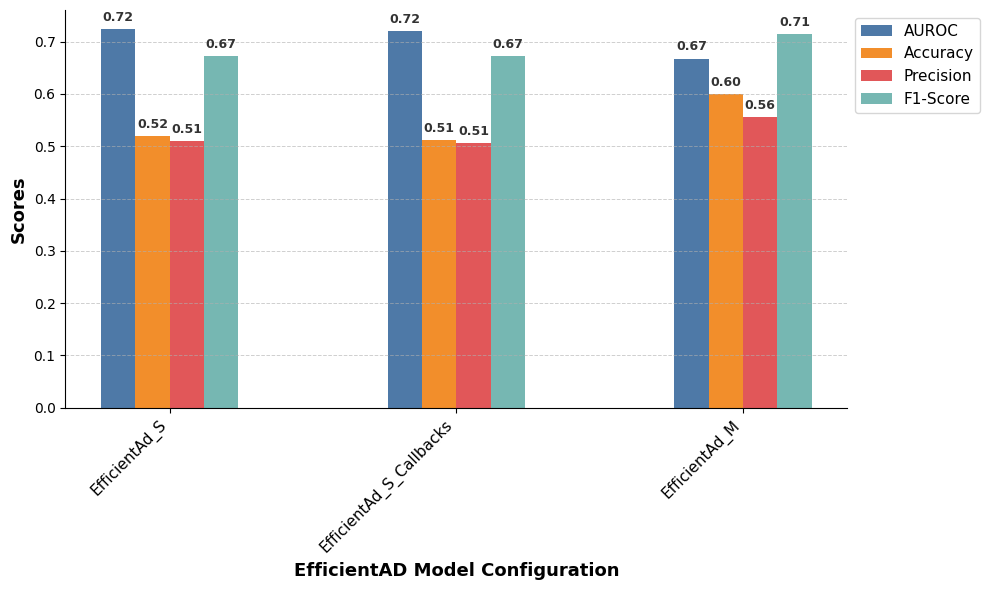
\includegraphics[width=1.2\linewidth]{Rohit_Master_Thesis//Images/efficientad_model_results.png}
    \caption{EfficientAD models result in bar-chart for different configurations used.}
    \label{fig:efficientad model results}
\end{figure}

While the EfficientAD model claims to outperform existing models, such as PatchCore\cite{roth2022totalrecallindustrialanomaly}, as given in the paper \cite{batzner2024efficientadaccuratevisualanomaly}, the experimental results conducted in this study suggest otherwise. The performance of EfficientAD was found to be suboptimal when evaluated on unseen data, as can be seen in the diagram \ref{fig:efficientad model results}. This section will discuss the results of different configurations in detail.

These experiments were carried out using three different configurations of the EfficientAD model. There are two sizes available for the model, which are EfficientAD\_S(small) and EfficientAD\_M(medium). The model size was constant for the first two configurations, but a callback mechanism was added in the second configuration. The Performance metrics used are the same as the rest of the models, namely \gls{auroc}, accuracy, precision, recall, and F1-score. Also, confusion matrices were generated to provide visual insights into how well the model performed in terms of classification.

In the first configuration, the base model (EfficientAdModelSize.S) was used without callbacks, as shown in the table \ref{tab:efficientad results}. This gave the \gls{auroc} of 0.7244. However, the model's accuracy was only 51.87\%, which clearly highlights its struggles in correctly classifying the majority of images. More specifically, out of 80 normal images, only 4 were correctly classified, with the remaining 76 being classified as abnormal, i.e., false positives. But on the other hand, the model performed quite well in detecting abnormal instances, with 79 out of 80 correctly classified as abnormal, resulting in a recall of 0.9875. But the precision is quite low at 0.5097, showing the imbalance between the true positives and false positives. The resulting F1-score was 0.6723, indicating a tendency towards recall, with the model detecting most anomalies but at the cost of misclassifying a large number of normal images as abnormal. Here, all the models were trained for 50 epochs except for when callbacks functionality is used. Then, it is trained until a condition is met.

\begin{table}[ht!]
    \centering
    \begin{tabular}{|l|c|c|c|c|c|}
        \hline
        \textbf{Model Size} & \textbf{AUROC} & \textbf{Accuracy(\%)} & \textbf{Precision} & \textbf{Recall} & \textbf{F1-Score} \\ \hline
        EfficientAd-S & 0.7244 & 51.88\% & 0.5097 & 0.9875 & 0.6723 \\ \hline
        EfficientAd-S (with callbacks) & 0.7203 & 51.25\% & 0.5063 & 1.0 & 0.6723 \\ \hline
        EfficientAd-M & 0.6678 & 60\% & 0.5556 & 1.0 & 0.7143 \\ \hline
    \end{tabular}
    \caption{Performance of EfficientAD Models with Different Sizes}
    \label{tab:efficientad results}
\end{table}

For the second configuration, the same model size (EfficientAdModelSize.S) was used, but ModelCheckpoint and EarlyStopping callbacks were added. The purpose of these callbacks was to improve the training process by ensuring that the model did not overfit and preserving the best weights during the training. Despite these improvements, the model's \gls{auroc} dropped slightly to 0.7203, and an overall accuracy of which relatively remained the same as before at 51.25\%, as seen in the table \ref{tab:efficientad results}. This result suggests that the callbacks had minimal to no impact on the model's ability to generalize on unseen data. In terms of precision and recall, the scores were 0.5063 and 1.0, respectively, this shows us that while the model was able to classify all the abnormal images correctly, but it struggled a lot at classifying the normal images correctly and ended up with lots of false positives. The confusion matrix values further confirm these findings, with only 2 normal samples being correctly classified, with the rest, 78 being misclassified as abnormal. The F1-score came out to be 0.6723, which is identical to that of the first configuration with no callbacks.

In the third and final configuration, the larger variant of the model (EfficientAdModelSize.M) was used. An \gls{auroc} score of 0.6678 was observed, which is less than the smaller model configurations scores, indicating a further decline in the model's ability to differentiate between normal and abnormal instances. Even then, an increase in overall accuracy was observed at 60\% with 16 normal samples correctly classified as normal, with 64 still being misclassified as shown in the confusion matrix \ref{fig:efficientad confusion matrix}. Although this is an improvement compared to other configurations, the model still struggles with a high number of false positives. The recall of 1.0 and increased precision of 0.5556 indicate an improved ability to correctly classify more normal images. The resulting F1-score is 0.7143, which is an improvement over smaller models, but it is still far from ideal.

\begin{figure}[H]
    \centering
    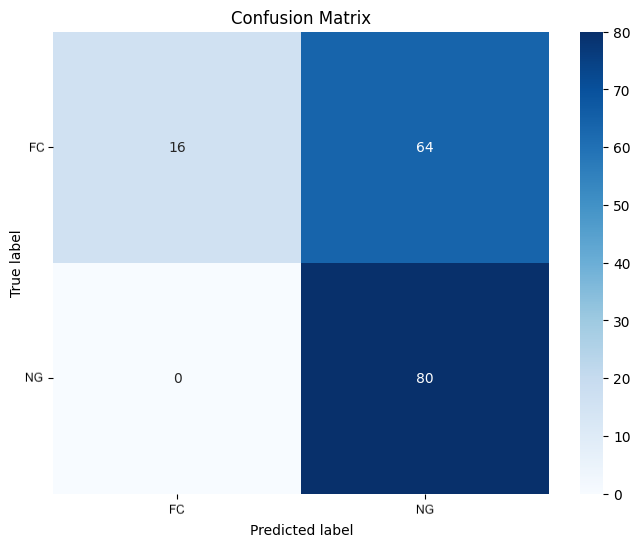
\includegraphics[width=1\linewidth]{Rohit_Master_Thesis//Images/efficientad_confusion_matrix_best.png}
    \caption{Confusion matrix for the best performing configuration for EfficientAD model with size EfficientAdModelSize.M, its accuracy is 60\%}
    \label{fig:efficientad confusion matrix}
\end{figure}




%\subsection{Layer wise performance comparison}

%\subsection{Performance on NG images}

%\subsection{Performance on FC images}

%\subsection{Discussion}

%5.2 The Case for Unsupervised Models: Patchcore's Robustness

%Patchcore emerged as the strongest unsupervised model, achieving 91.25% accuracy and an AUROC of 0.9271. One of the key strengths of Patchcore is its ability to function effectively without requiring labeled anomaly data, making it highly suitable for real-world industrial applications. This model leverages feature representations from multiple layers of the network (layer1 and layer2 in its best configuration), allowing it to capture complex anomalies across different scales and granularities.

%Patchcore's F1 score of 0.9434 further underscores its effectiveness in balancing precision and recall, ensuring that false positives and false negatives are minimized. From a practical standpoint, this makes Patchcore a strong candidate for use in settings where it is crucial to minimize missed anomalies (false negatives) but also to reduce the burden of excessive false positives, which can lead to unnecessary inspections or interventions.

%Additionally, Patchcore's confusion matrix reflects a well-rounded performance with only 2 false negatives and 12 false positives, highlighting its ability to handle both normal and abnormal cases effectively. This is especially important in applications such as predictive maintenance, where the cost of missing a potential failure is high, and unnecessary repairs due to false positives can also be costly.

%Conclusion: Patchcore's robust performance without the need for labeled data makes it an ideal choice for unsupervised anomaly detection tasks, especially in industries like manufacturing, medical diagnostics, and predictive maintenance, where labeling anomalies is often impractical.

% In discussions explain also the difference between scoring type fre and nll
% In discussion also discuss why was the recall for most part 1.0

%Probably for discussion section(remember to paraphrase)
%Explanation of Results

%YOLOv8-M strikes a balance between computational efficiency and accuracy. The model achieves 93.75\% accuracy, which is competitive given its smaller architecture compared to YOLOv8-L. The slightly lower performance is expected due to YOLOv8-M’s reduced depth and number of parameters, which limits its ability to capture as many intricate patterns in the data as YOLOv8-L. However, YOLOv8-M’s simpler structure makes it faster and more computationally efficient, making it suitable for tasks where real-time performance and resource limitations are important.

%Model Comparison and Insights
%YOLOv8-L outperforms YOLOv8-M by achieving 95\% accuracy, compared to YOLOv8-M’s 93.75\%. This difference in performance can be attributed to the larger number of layers and parameters in YOLOv8-L, which allows it to capture more detailed features from the dataset. YOLOv8-L’s larger architecture is particularly beneficial for classification tasks that involve complex patterns or subtle differences between classes, making it a better choice for applications where accuracy is critical.

%However, YOLOv8-M offers significant advantages in terms of speed and computational efficiency. Despite having fewer layers, YOLOv8-M achieves strong results, making it a good option for scenarios where real-time inference is necessary or where computational resources are limited. The slight trade-off in accuracy is reasonable given the gains in efficiency, making YOLOv8-M ideal for environments where fast processing is prioritized over achieving the highest possible accuracy.

%Probably for discussion section(remember to paraphrase)
%Explanation of Results
%The performance of YOLOv8-L is in line with its design as a larger, more powerful model. The depth and complexity of the YOLOv8-L architecture allow it to capture a wide variety of patterns and features in the data, leading to its high precision and recall. The non-maximum suppression (NMS) technique used in YOLOv8 helps further refine the predictions by ensuring that overlapping bounding boxes are filtered, resulting in more accurate object classification. Additionally, YOLOv8-L's anchor-free detection mechanism improves its ability to generalize across objects of various sizes, contributing to its robustness in detecting NG and FC items.


% In DFM resnet results why changing the PCA_level and scoring type to fre resulted in better results?

%Discussion of Results and Insights for DFM

%The results of the experiments provide valuable insights into how the choice of backbone network, feature extraction layer, and scoring method influence the performance of the DFM model. Across all configurations, the model demonstrated high recall values, indicating its strong ability to detect anomalous samples. However, the key challenge in most configurations was improving precision, as many configurations suffered from high false-positive rates. This imbalance between precision and recall was most noticeable in configurations that used higher-level feature layers, such as layer4 in ResNet50, which may have caused the model to focus on abstract features less relevant for anomaly detection.

%The use of PCA for dimensionality reduction also played a crucial role in balancing the model’s performance. A PCA level of 0.97 generally provided a good balance between computational efficiency and information retention, while increasing the PCA level to 0.995 resulted in slightly higher overfitting and a decrease in precision. Additionally, the frequentist score type consistently outperformed the negative log-likelihood score in anomaly detection tasks, as it provided a more robust measure of the distance between the new data points and the normal data distribution.

%In conclusion, the DFM model’s performance varied significantly across different configurations. The best-performing setup used DenseNet169 with features extracted from DenseBlock3, a PCA level of 0.97, and the frequentist score type, achieving a balance between high precision and recall while maintaining a high sensitivity to anomalies. Future work could explore the integration of attention mechanisms or ensemble methods to further improve precision and reduce the false-positive rate, particularly in configurations that show a tendency to misclassify normal samples as anomalies.

%I can add diagram showing the performance according to layers

%DFKDE

%Discussion of Results Based on Backbone
%The results of the experiments show that the choice of backbone architecture and the layer from which features are extracted significantly affect the performance of the DFKDE model. Across the ResNet18 experiments, the best results were obtained when extracting features from layer2 or layer3, as these layers provided a balance between precision and recall. Layer1, which captures low-level features, produced the lowest precision and accuracy, likely due to its inability to capture the necessary high-level patterns required for accurate anomaly detection.

%In contrast, the Wide-ResNet50-2 backbone consistently outperformed ResNet18 in terms of AUROC, suggesting that the wider architecture was more effective at capturing subtle differences between normal and anomalous data. However, the performance of the Wide-ResNet50-2 model was highly dependent on the number of principal components retained during the PCA step. Retaining too many components, as seen in the final experiment, introduced noise that reduced precision, while using fewer components provided a better balance between recall and precision.

%In conclusion, the DFKDE model's performance is sensitive to both the choice of backbone architecture and the feature extraction layer. While ResNet18 provides satisfactory results, Wide-ResNet50-2 offers better overall performance, especially when mid-level features are extracted from layer2. The trade-off between precision and recall is heavily influenced by the layer used for feature extraction, and careful tuning of the PCA level is essential for optimizing the model’s anomaly detection capabilities. These findings suggest that DFKDE is a flexible and powerful anomaly detection framework, with its performance closely tied to the choices made during the feature extraction and dimensionality reduction processes.

%EfficientAD Discussion
%The results of the experiments demonstrate that while EfficientAD is designed for efficiency, it struggles with the accuracy and precision required for real-world anomaly detection tasks. In all three configurations, the model exhibited high recall, meaning that it was consistently able to identify abnormal instances. This is an important quality for anomaly detection, particularly in applications where it is critical to catch every possible anomaly. However, the model’s precision was consistently low across all configurations, highlighting a major issue: a significant number of normal samples were misclassified as anomalies.

%One of the key reasons for this performance discrepancy could be the model's underlying architecture. EfficientAD's focus on reducing computational complexity through the use of a smaller student model might have come at the cost of reduced representational capacity. The model's teacher-student framework is designed to ensure that the student model can mimic the teacher’s outputs, but this transfer of knowledge might not be as effective when it comes to detecting subtle variations between normal and abnormal instances. In contrast, PatchCore, which relies on more robust and larger feature representations, seems to be better suited for capturing these nuances, which could explain why it outperformed EfficientAD in these experiments.

%Another factor to consider is the dataset used in these experiments. While EfficientAD was trained and tested on a large-scale dataset like Imagenet, the generalization capabilities of the model may be limited when applied to unseen data. Anomaly detection is highly sensitive to the specific characteristics of the dataset, and a model that performs well on one dataset may not necessarily generalize to others. In this case, the dataset used for testing may contain subtle differences from the training data, which EfficientAD was unable to capture, leading to a higher rate of misclassification.

%PatchCore’s superior performance can also be attributed to its underlying architectural advantages. PatchCore uses a memory bank of features extracted from the training data, which allows it to compare new samples against a more diverse and representative set of normal instances. This approach enables PatchCore to better detect subtle anomalies that might be overlooked by more simplified models like EfficientAD. In contrast, EfficientAD’s reliance on a student-teacher framework, while computationally efficient, may result in the loss of critical information that is necessary for accurate anomaly detection.

%Additionally, PatchCore’s design allows for better feature extraction, as it does not reduce the complexity of the model as much as EfficientAD. This could explain why, despite being an older model, PatchCore consistently outperforms EfficientAD in terms of both precision and recall. EfficientAD's strength lies in its ability to operate in real-time and on resource-constrained devices, but this efficiency comes with trade-offs in accuracy that may not be acceptable for certain applications.

%In conclusion, while EfficientAD offers an attractive solution for real-time anomaly detection in resource-constrained environments, it faces significant challenges in achieving the level of accuracy and precision required for high-stakes applications. The model’s high recall is commendable, but its low precision indicates that it generates too many false positives, which could limit its usability in certain domains. PatchCore, on the other hand, continues to outperform newer models like EfficientAD due to its more robust feature extraction and memory-based approach. As such, the choice between EfficientAD and PatchCore ultimately depends on the specific requirements of the application, with EfficientAD being more suited for real-time tasks where speed is of the essence, and PatchCore being the better choice for tasks where accuracy is paramount.


%Fastflow Discussion and Insights

%Across the experiments, we observe that increasing model complexity through the use of wider or deeper backbones generally improves anomaly detection, though at the cost of classifying normal images less accurately. The backbone architectures like Wide-ResNet50-2, DeiT, and CaiT each offered unique advantages. Wide-ResNet50-2, with its increased width, struggled with balancing normal and anomalous classifications. DeiT, with its transformer-based approach, improved classification of normal samples, and CaiT’s deep attention mechanism allowed for even more nuanced understanding of the image space, reflected by its superior AUROC.

%FastFlow’s reliance on normalizing flows works well in modeling the distribution of normal images but can struggle when anomalies are not sufficiently distinct in the feature space. This is evident from the precision-recall tradeoff seen across all experiments: while recall was consistently high, precision fluctuated, highlighting that misclassifications of normal samples as abnormal remained a challenge.

%Incorporating pre-trained models provided a solid foundation, though the results suggest that the specific nature of anomaly detection tasks may require fine-tuning of these pre-trained backbones for optimal performance. Training for additional epochs, as seen in Experiments 3 through 5, consistently improved results, implying that FastFlow benefits from extended training periods to better capture the feature space of normal images.

%These findings highlight that while FastFlow is effective at detecting anomalies, future work could focus on balancing the precision-recall tradeoff, perhaps through more advanced fine-tuning techniques or hybrid architectures that combine the benefits of convolutional networks and transformers, or more carefully tuned flow step configurations.



